% Chapter 1
% Main chapter title
\chapter{The current state of the subject.}% For referencing the chapter elsewhere, use \ref{Chapter1}
\label{Chapter1}
% This is for the header on each page - perhaps a shortened title
\lhead{Chapter 1. \emph{The current state of the subject}} 

Up to now, the methods used for analysis of electrophysical properties
of MOS structures are based on the assumption that the distribution of
impurities in the substrate is homogeneous. This issue was addressed
by the Department of Microelectronics within the government research
projects~\cite{1.1,1.2} and PhD thesis~\cite{1.5,1.6,1.7,1.8}. These
works provide the necessary overview of the solutions for the problems
globally and also in our department. Whereas at present in the
manufacture of unipolar integrated circuits using ion implantation for
control the electrical properties of integrated components, it is
desirable to control the properties of semiconductor structures to
know the parameters of MOS structures with inhomogeneous subsidy
substrate. For this purpose was research task Electrophysical
properties of microelectronic structures~\cite{1.3,1.4} focused on the
development of diagnostic methods for study of the properties of
technological processes using MOS structures with inhomogeneous
subsidy impurities and their application to solving problems of
Czech-Slovak semiconductor industry. From this target of the government
research project resulted the focus of the presented thesis. The need
to address this issue is also based on the fact that up till now this
issue, as far as we known, has never been studied here. Additionally,
the issue was extended to the research of electro-physical parameters'
homogeneity of MOS structures on silicon substrate, which is
particularly serious in the light of the process quality improvement
of forming a semiconductor structures and integrated circuits by
planar technology. Based on the foregoing, we list later in this
chapter only the most necessary knowledge needed to deal with the
issues.

\section{Basics of the MOS structure.}

MOS structure forms a simple test structure. Almost all of its
electrical properties can be examined by measurements of this
structure. Convenience of the MOS structure lies in the ease of
preparation and analysis of its features. The simplicity of analysis
follows that analyzed system is in thermal equilibrium and
one-dimensional approach is sufficiently accurate in most
cases. Properties of the $SiO_2$ volume, its interfaces with
semiconductor and metal, as well as properties of the subsurface area
of semiconductor can be examined by electrical measurements of MOS
structure.

\section{Ideal MOS structure.}\index{MOS!ideal structure}

MOS structure can be considered a dipole, which equivalent scheme can
be thought of as a serial connection of voltage-independent capacity
of the oxide $C_{ox}$ and capacity of the space charge region (SCR)
$C_{sc}(\varphi_{s})$, which is a function of the surface potential of
the semiconductor. Then for the capacity of MOS structure is
valid~\cite{I.1}

\begin{equation}\label{eq:1.1}
  \frac{1}{C_{mos}(V_g)} = \frac{1}{C_{ox}} + \frac{1}{C_{sc}(\varphi_s)}
\end{equation}

Following simplistic assumptions, that define ideal MOS structure, can
be used when analyzing the MOS structure:

\begin{itemize}
\item the density of interface traps $Si-SiO_2$ is equal zero
\item there are no charges in the insulator $SiO_2$
\item the difference in the output potential of the metal and
  semiconductor is equal zero
\item equation $V_{g}=V_{ox}+\varphi_{s}$ is valid.
\end{itemize}

\noindent Depending on the gate voltage operating modes of MOS
structure can be distinguished:

\begin{itemize}
\item enhancement mode
\item flat band mode
\item depletion mode and inversion (deep depletion).
\end{itemize}

\section{Capacitor characteristics of ideal MOS structure.}\index{MOS!ideal structure}

For all of these cases one-dimensional Poisson equation is valid in
the semiconductor

\begin{equation}\label{eq:1.2}\index{Poisson equation}
  \frac{d^2\varphi}{dx^2} = -\frac{q}{\varepsilon}(p-n+N_{p}-N_{A})
\end{equation}

which determines the course of the electrical potential $\varphi$ as a
function of the distance from the surface of the semiconductor
$x$. Equation~\ref{eq:1.2} can be solved analytically only for certain
special cases of the impurities concentration profile, and, in
general, numerical methods must be used~\cite{1.9,1.10}. Then, for
known profile of the concentration impurities in semiconductor an
electric potential in the semiconductor can be obtained, where
potential on the gate is the parameter which defines the state of the
MOS structure. For further clarification of physical processes in the
MOS structure in the transition from accumulation to inversion, or
deep depletion, we solved the equation~\ref{eq:1.2}, where by
appropriate variation of the parameter $V_g$ both surface
potential~\index{surface potential} $\varphi_{s}(V_g)$ and capacity of
MOS structure $C_{MOS}(V_g)$ can be calculated as a function of the
gate voltage (see Appendix~\ref{app:AppendixA}).

\begin{figure}[h!]\centering
  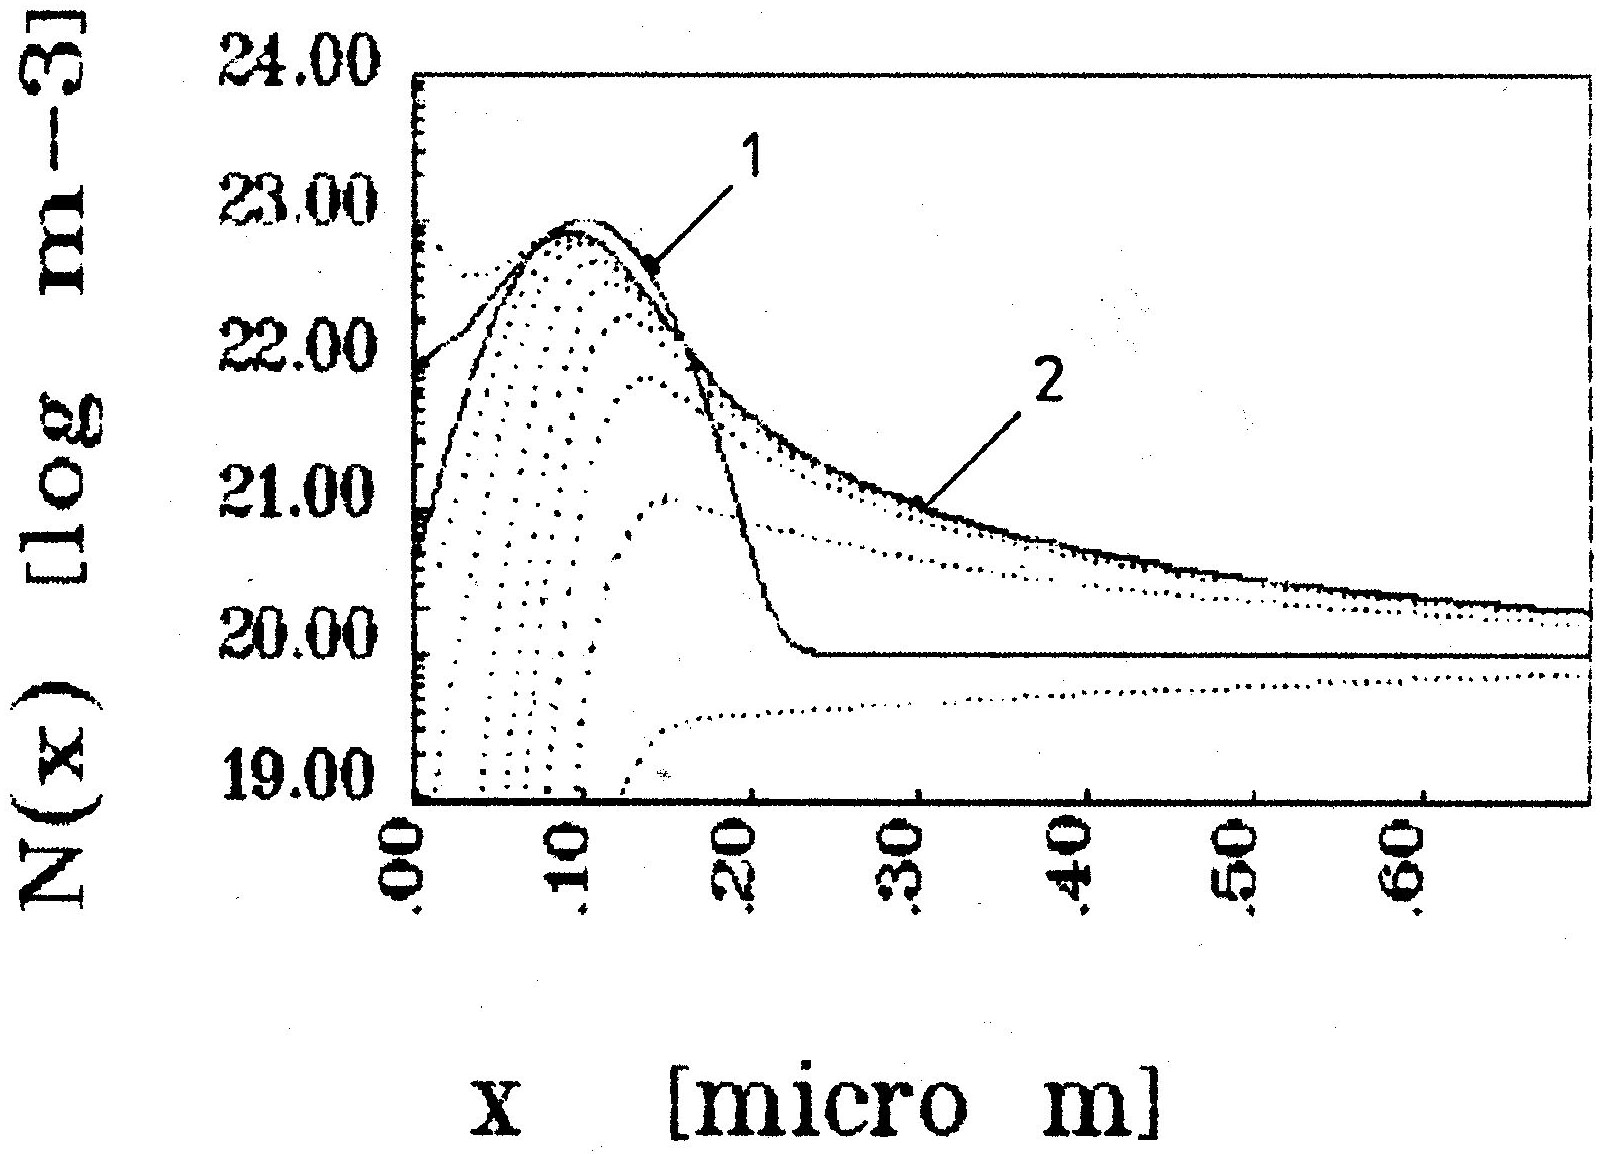
\includegraphics{Figures/fig-1-1.eps}% chktex-file 8
  \caption[Concentration of dopant in the subsurface of the
    semiconductor] {Concentration of dopant in the subsurface of the
    semiconductor simulated by Gaussian distribution~\cite{1.11} with
    the following parameters $R_p=0.1 \mu{m}$;
    $\Delta{R_p}=0.03\mu{m}$; $N_{\max}=10^{23} m^{-3}$;
    $N_{bulk}=10^{20} m^{-3}$ (indicated by a solid line 1). The
    profile of the majority charge carriers for $V_g=0$ (indicated by
    a solid line 2). The dotted line shows profiles of the
    concentrations of majority carriers for various gate voltages
    different from zero. State of thermodynamic equilibrium between
    the distribution of dopant and charge carriers is described in
    Appendix~\ref{app:AppendixD}.}\label{fig:1.1}
\end{figure}

\par Figure~\ref{fig:1.1} shows the profile of the dopant
concentration in semiconductor (simulated by Gaussian function) and
profiles of majority charge carriers for states of the structure
varying from enhancement to inversion, depicting the process of
depletion of the semiconductor subsurface. It can be seen, that the
profile of the concentration of majority carriers in implanted field
enter the maximum and then decreases toward the concentration of the
substrate, which is reached at a ground potential point. Also obvious
is the difference between the concentrations of dopant and the
concentration of majority charge carriers in the state of
thermodynamic equilibrium for zero gate voltage, which results indue
to diffusion of majority charge carriers.

\newpage
\begin{figure}[h!]\centering
  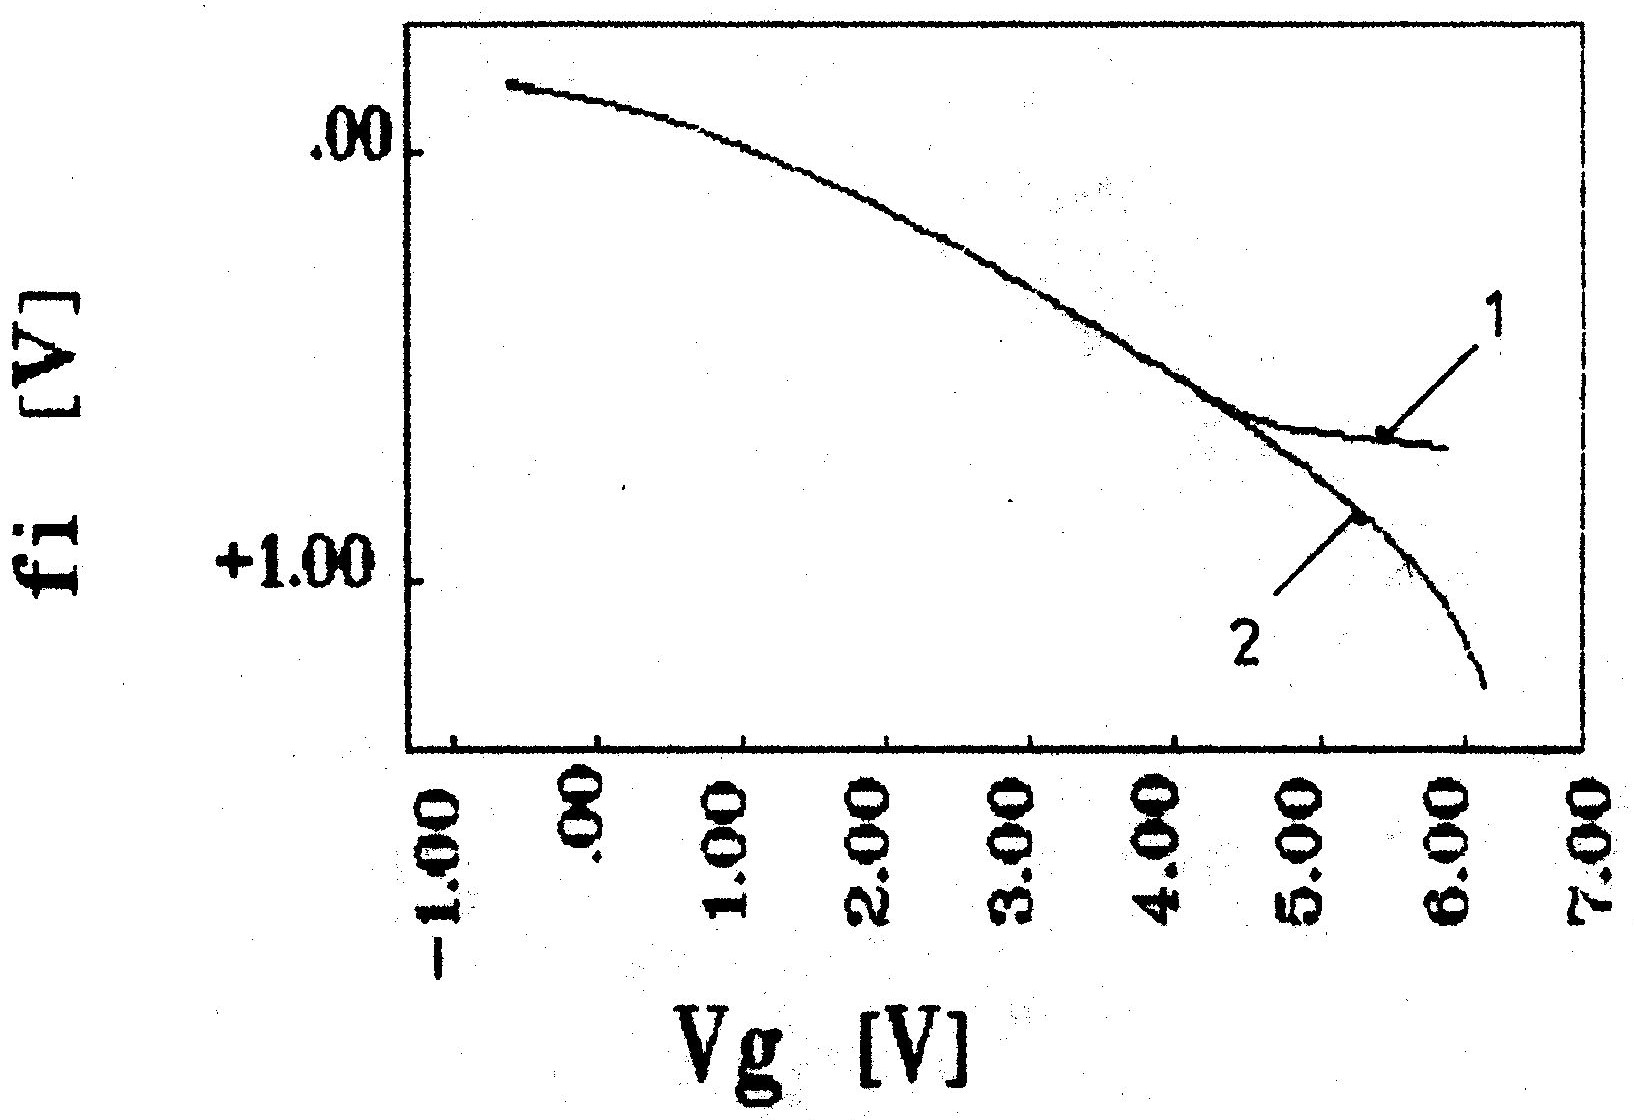
\includegraphics{Figures/fig-1-2.eps}
  \caption[Surface potential $\varphi_s(V_g)$ as a function of the
    gate voltage]{Surface potential $\varphi_s(V_g)$ as a function of
    the gate voltage for low frequency (LF) and high frequency (HF)
    measurement (depicted 1) and measurement in deep depletion
    (depicted 2).}\label{fig:1.2}
\end{figure}

\begin{figure}[h!]\centering
  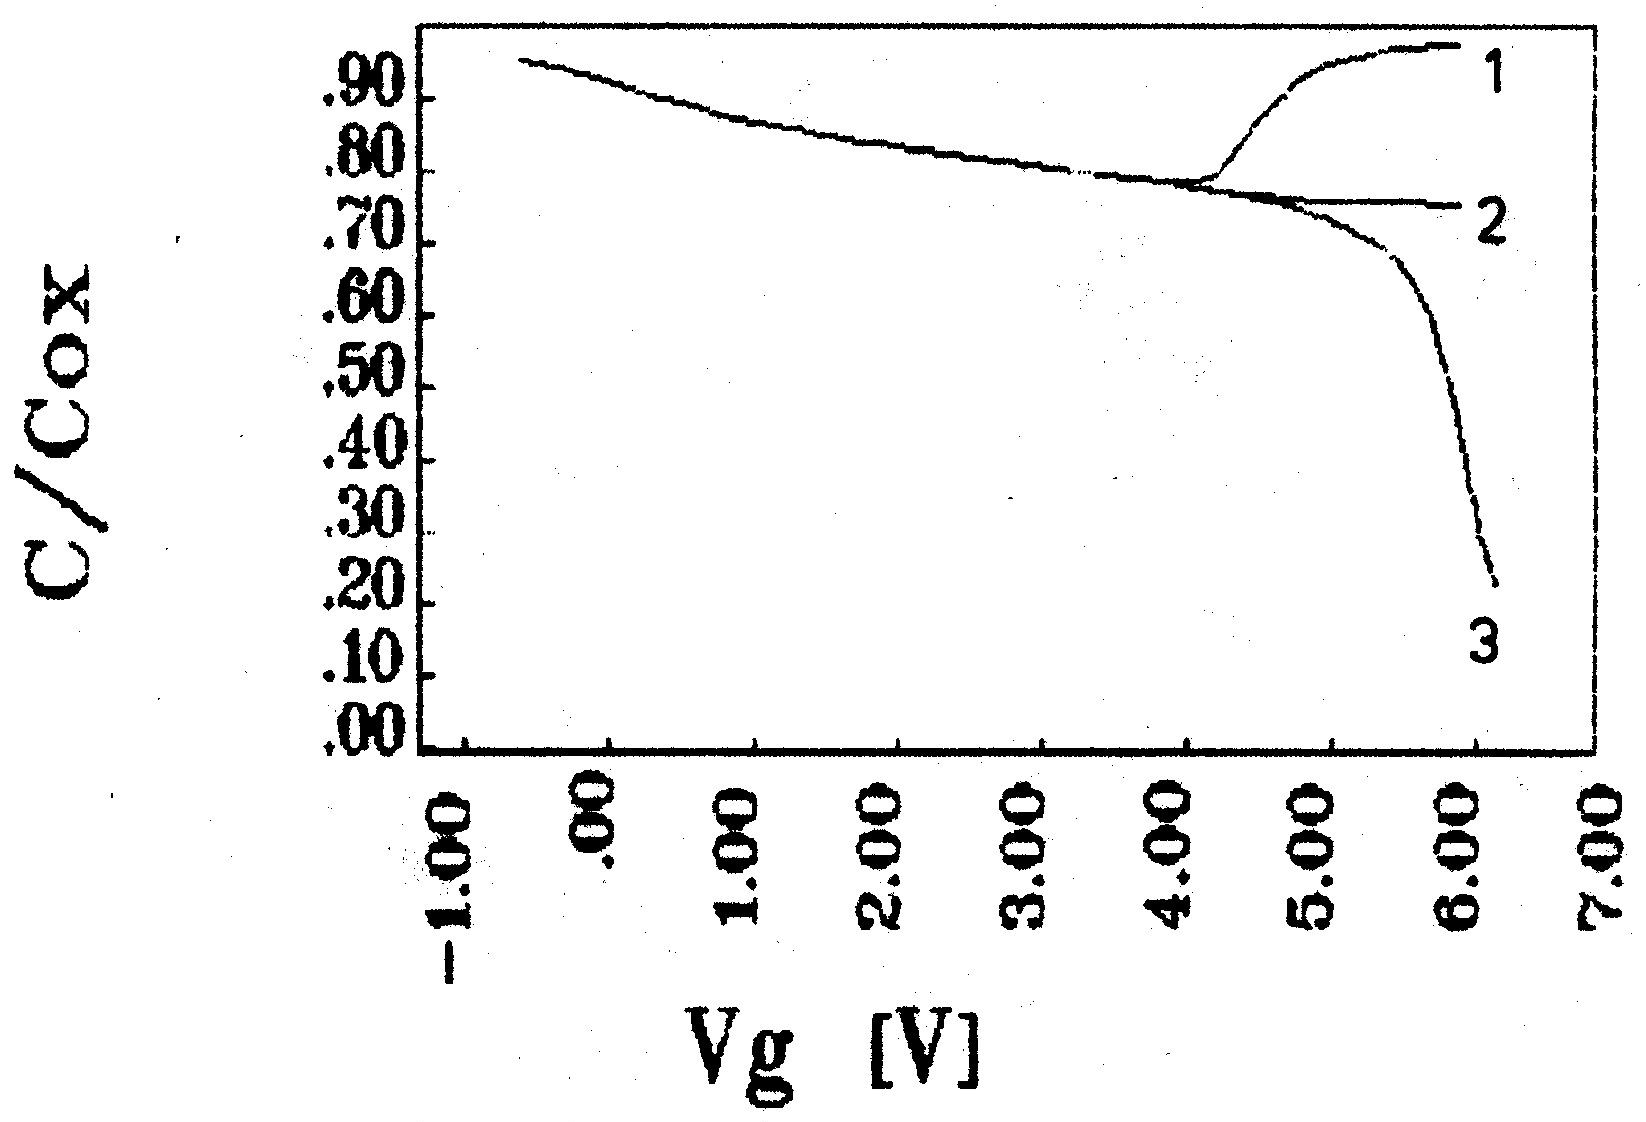
\includegraphics{Figures/fig-1-3.eps}
  \caption[Profile of the capacity of the MOS structure depending on
    the gate voltage]{Profile of the capacity of the MOS structure
    depending on the gate voltage for low frequency measurement
    (depicted 1), high frequency measurement (depicted 2) and
    measurement in deep depletion (depicted 3).}\label{fig:1.3}
\end{figure}

\par Figure~\ref{fig:1.2} shows surface potential for various
measurements of the MOS structure. In the enhancement and depletion
both curves are identical. From the beginning of the inversion the
surface potential stabilizes for LF and HF measurements as a result of
the creation of the inversion layer. The curve of deep depletion
further declines. This state will be terminated by the breakdown in a
real structure.

\par Figure~\ref{fig:1.3} shows Capacitance-Voltage profiles of the
MOS structure. All three curves are identical in enhancement and
depletion (profiles of the surface potential are also identical). In
this section the capacity declines slowly, because the space charge
region expands to the region with high concentration of the
dopant~\ref{fig:1.1}. From the beginning of the inversion the the
curves depart. Low frequency curve, which detects the inversion layer
rises toward the capacity of the silica. High frequency curve doesn't
detect the inversion layer, because the minority charge carriers are
not able to follow the high frequency measurement signal. However the
capacity doesn't decline any further, because with the increasing of
the gate voltage increases mostly the concentration of the minority
charge carriers in the inversion layer and the space charge region
doesn't expand any further.

\par No inversion layer is created in deep depletion and with the
increasing gate voltage the space charge region expands and capacity
declines. Figure~\ref{fig:1.3} shows, that after having passed the
section with the high concentration of dopant the curve of deep
depletion starts to decline faster.

\section{Real MOS structure.}\index{MOS!real structure}

The difference of ideal and real MOS structure was treated
in~\cite{1.12} and here we introduce only a review. Electrical
properties of real MOS structure are different from the ideal model
mainly due to the defect charges in the oxide layer and in its
interface with the semiconductor and metal, which can be divided into
the following groups:

\begin{itemize}
\item charge of the mobile ions in the oxide layer - $Q_{m}$
\item charge of the ionized traps in the oxide - $Q_{ox}$
\item fixed charge at the interface $Si-SiO_2$, due to the
  non-stoichiometric composition of the phase transition - $Q_f$
\item charge of the traps at the interface $Si-SiO_2$ - $Q_{it}$
\end{itemize}

\par At the same time the electrical properties of MOS structure are
also affected by the difference in work function between metal and
semiconductor, $\varphi_{ms}\neq{0}$. In addition to the defect
charges geometrical imperfections of the structure, changing thickness
of the insulating layer and non-planarity of the interface $Si-SiO_2$
influence electrical properties of MOS structure. The transition to a
very large integration requires to address the micro-defects in the
volume of silicon, which represent a disorder of the crystal lattice
resulted in the production of the mono-crystal, its primary treatment
to the form of a silicon wafer and during the technological processing
of the components. If those defects are found in the area of
functional parts, they have adverse effects on electrical
parameters. However, micro-defects of suitable size in the volume of
semiconductor produce effects which are often used to create so-called
denuded zone. Deliberate creation of micro-defects in the volume of
semiconductor by implantation of carbon and subsequent heating may
significantly increase the lifetime of the minority charge
carriers~\cite{1.13}. In~\cite{1.14} authors clearly displayed with
laser scanning tomography a denuded zone at silicon surface formed by
microprecipitates $SiO_x$. Microprecipitates in the volume of the
semiconductor, created with oxygen and appropriate heat-processing,
are also seen from the images.

\begin{thebibliography}{}
\bibitem[1.1]{1.1} Csabay O. et al: Výskum štruktúr MIS a
  pasivácie. Záverečná správa štátnej výskumnej úlohy III-4-3/2. EF
  SVŠT, Bratislava 1980.
\bibitem[1.2]{1.2} Csabay O. et al: Výskum elektrofyzikálnych
  vlastností mikroelektronických unipolárnych štruktúr. Záverečná
  správa štátnej výskumnej úlohy III-6-1/13. EF SVŠT, Bratislava 1985.
\bibitem[1.3]{1.3} Csabay O., Botka V. et al: Elektrofyzikálne
  vlastnosti mikroelektronických štruktúr. Priebežná správa Štátnej
  výskumnej úlohy III-7-2/04. Katedra mikroelektroniky EF SVŠT,
  Bratislava 1988.
\bibitem[1.4]{1.4} Csabay O., Botka V. et al: Elektrofyzikálne
  vlastnosti mikroelektronických štruktúr. Záverečná správa Štátnej
  výskumnej úlohy III-7-2/04, Katedra mikroelektroniky EF SVŠT,
  Bratislava 1990.
\bibitem[1.5]{1.5} Žiska M.: Kandidátska dizertačná práca. Katedra
  mikroelektroniky EF SVŠT, Bratislava 1985.
\bibitem[1.6]{1.6} Harmatha L.: Výskum vlastností štruktúry MIS v
  nerovnovážnom stave kapacitnou metódou. Kandidátska dizertačná
  práca. Katedra mikroelektroniky EF SVŠT, Bratislava 1983.
\bibitem[1.7]{1.7} Valehrachová D.: Kandidátska dizertačná
  práca. Katedra mikroelektroniky EF SVŠT, Bratislava
\bibitem[1.8]{1.8} Kinder R.: Príspevok ku skúmaniu koncentračných
  profilov implantovaných vrstiev. Kandidátska dizertačná práca. EF
  SVŠT Bratislava 1984.
\bibitem[1.9]{1.9}
  \href{http://ieeexplore.ieee.org/xpl/articleDetails.jsp?arnumber=4236397&filter\%3DAND\%28p_IS_Number\%3A4236383\%29}
  {El- Sissi H., Cobbold R.S.C.: Electronic Letters 25 (1973) s.594.}
\bibitem[1.10]{1.10} 
  \href{http://ieeexplore.ieee.org/xpl/freeabs_all.jsp?arnumber=1477966}
  {Klopfenstein R.W., Wu C.P.: IEEE Trans.\ on electron.\ devices} ED-22 (1975) s.329.
\bibitem[1.11]{1.11}
  \href{http://www.springer.com/us/book/9783519032069}
  {Ryssel H., Ruge I.: Ionenimplantation. Stuttgart 1978}
\bibitem[1.12]{1.12} Csabay O.: Niektoré technologické a fyzikálne
  problémy štruktúr MIS\@. Doktorská dizertačná práca. Katedra
  mikroelektroniky, EF SVŠT, Bratislava 1986.
\bibitem[1.13]{1.13}
  \href{http://ieeexplore.ieee.org/xpl/articleDetails.jsp?arnumber=59491&filter\%3DAND\%28p_IS_Number\%3A2166\%29\%26pageNumber\%3D2}
  {Skorupa W., Kogler R.: Electronics Letters Vol.25 (1989) s.1898.}
\bibitem[1.14]{1.14}
  \href{http://ieeexplore.ieee.org/xpl/login.jsp?tp=&arnumber=18492&url=http\%3A\%2F\%2Fieeexplore.ieee.org\%2Fxpls\%2Fabs_all.jsp\%3Farnumber\%3D18492}
  {Gall P. at al.: Electronics Letters Vol.25 (1989) s.429.}
\end{thebibliography}
